\documentclass[titlepage]{article}
\usepackage{babel}
\usepackage{amsmath}
\usepackage{amssymb}
\usepackage{amsthm}
\usepackage{stmaryrd} %ligtning

\usepackage{tabto} %tabulator mit \tab
\usepackage{tikz}
\usetikzlibrary{automata, arrows.meta, positioning, shadows, shapes.geometric} % automaten zeichnen
\usepackage[utf8]{inputenc}
\pagestyle{plain}
\pagenumbering{arabic}
\renewcommand{\arraystretch}{1.3} %vertikaler abstand von tabellen
\usepackage[left=20mm, right=15mm, top=25mm, bottom=7mm, paper=a4paper]{geometry}

\renewcommand{\contentsname}{Inhaltsverzeichnis}
\renewcommand{\]}{\right]}
\renewcommand{\[}{\left[}
\renewcommand{\)}{\right)}
\renewcommand{\(}{\left(}
\renewcommand{\|}{\;|\;}
\newcommand{\n}{\newline}
\renewcommand{\l}{\linebreak}



\begin{document}\begingroup\let\clearpage\relax
	%header
	\begin{center}
	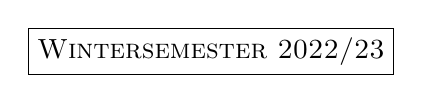
\begin{tikzpicture}
		\draw (0,0) node[draw, rectangle]{\textsc{Wintersemester 2022/23}};
	\end{tikzpicture}
	\hrulefill\\
	\begin{center}
		\LARGE\textsc{Automaten und Berechenbarkeit - Übung 05} \normalsize\\
	\end{center}
	\hrulefill
	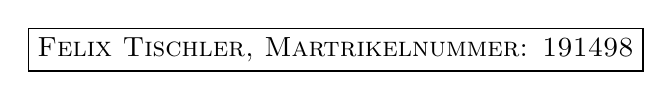
\begin{tikzpicture}
		\draw (0,0) node[draw, rectangle]{\textsc{Felix Tischler, Martrikelnummer: 191498}};
	\end{tikzpicture}
	\date{\today}
\end{center}
	
	%task one
	\section*{Aufgabe 1}
	Wir betrachten die Sprache $L=\{a^ib^jc^k\mid i,j,k\in\mathbb{N},i=0\;oder\;j=k\}$
		\paragraph{(a)} Geben Sie eine kontextfreie Grammatik an, die $L$ erzeugt.
		Ann: sei $L_1\in CF\Rightarrow\exists n\in\mathbb{N}:\forall x\in L_1\;mit\;\mid x\mid\ge n:\exists x=uv_1\tilde{v}v_2w\;mit\;\mid v_1v_2\mid\ge1,\mid v_1\tilde{v}v_2\mid\le n:\forall i\in\mathbb{N}:uv_1^i\tilde{v}v_2^iw\in L_1$:
\noindent\\\\
\begin{math}
	Wähle\;x=a^nb^{n+1}c^{n+2},\;mit\\\\
	u=a^n\\
	v_1=b^{k_1}\\
	\tilde{v}=b\\
	v_2=b^{k_2}\\
	w=bc^n\\
	\;mit\;k_1+k_2=n-1\\\\
	\overset{i=0}{\Longrightarrow}a^nb^{n+1-k_1-k_2}c^{n+2}\overset{\mid v_1v_2\mid\ge1}{\Longrightarrow}L_1\notin CF
\end{math}
		\paragraph{(b)} L ist nicht regulär. Begründen Sie, dass man durch direkte Anwendung des Pumping-\\Lemmas für reguläre Sprachen \textbf{nicht} zeigen kann, dass $L$ nicht regulär ist.\\\\
		$G_2=(\{a,b,c\},\{S,R\},S,R)$
\begin{align*}
	Mit\;R=:
	\begin{cases}
		S&\rightarrow\quad Rc\\
		R&\rightarrow\quad aRc\mid Rbc\mid a\mid b
	\end{cases}
\end{align*}
		\paragraph{(c)} Zeigen Sie, dass $L$ nicht regulär ist.
		Ann: sei $L_3\in CF\Rightarrow\exists n\in\mathbb{N}:\forall x\in L_3\;mit\;\mid x\mid\ge n:\exists x=uv_1\tilde{v}v_2w\;mit\;\mid v_1v_2\mid\ge1,\mid v_1\tilde{v}v_2\mid\le n:\forall i\in\mathbb{N}:uv_1^i\tilde{v}v_2^iw\in L_3$:
\noindent\\\\
\begin{math}
	Wähle\;x=a^nb^nc^{n^2},\;mit\\\\
	u=a^{n-k_1-k_2-k_3}\\
	v_1=a^{k_1}\\
	\tilde{v}=a^{k_2}\\
	v_2=a^{k_3}\\
	w=b^nc^{n^2}\\
	mit\;k_1+k_2+k_3\le n\\\\
	\overset{i=0}{\Longrightarrow}a^{n-k_1-k_3}b^nc^{n^2}\Rightarrow L_3\notin CF
	\\\\Oder:\\\\
	u=a^n\\
	v_1=b^{k_1}\\
	\tilde{v}=b^{k_2}\\
	v_2=b^{k_3}\\
	w=c^{n^2}\\
	mit\;k_1+k_2+k_3=n\\\\
	\overset{i=0}{\Longrightarrow}a^nb^{k_2}c^{n^2}\Rightarrow L_3\notin CF
	\\\\Oder:\\\\
	u=a^nb^n\\
	v_1=c^{k_1}\\
	\tilde{v}=c^{k_2}\\
	v_2=c^{k_3}\\
	w=c^{n^2-k_1-k_2-k_3}\\
	mit\;k_1+k_2+k_3\le n\\\\
	\overset{i=0}{\Longrightarrow}a^nb^nc^{n^2-k_1-k_3}\Rightarrow L_3\notin CF
\end{math}\\
Man könnte auch noch in a und b oder in b und c pumpen, ebenso würde man durch pumpen ein nicht akzeptierbares Wort erhalten.
	\section*{Aufgabe 2}Gegeben sind die Sprachen $L_1=\{w\in\{0,1\}^*\mid\#_1(w)\equiv0\mod3\}$ und\\ $L_2=\{w\in\{0,1\}^*\mid w\text{ enthält das Teilwort 011 nicht}\}.$ \\Konstruieren Sie einen DFA $M$ mit $L(M)=\overline{L_1}\cap L_2$
	\begin{center}
	$M=(\{a,b\},\{A,B,\qedsymbol\},\{Z_0,Z_{ende}\},\delta,Z_0,\{Z_{Ende}\})$\\
\end{center}
Mit:
\begin{center}
	\begin{align*}
		\begin{cases}
			(Z_0,a,\qedsymbol)$&\rightarrow\quad$(Z_0,A\qedsymbol)\\
			(Z_0,a,A)$&\rightarrow\quad$(Z_0,AA)\\
			(Z_0,a,B)$&\rightarrow\quad$(Z_0,\lambda)\\
			(Z_0,\lambda,\qedsymbol)$&\rightarrow\quad$(Z_{ende})\\
			(Z_0,b,\qedsymbol)$&\rightarrow\quad$(Z_0,B\qedsymbol)\\
			(Z_0,b,A)$&\rightarrow\quad$(Z_0,\lambda)\\
			(Z_0,b,B)$&\rightarrow\quad$(Z_0,BB)
		\end{cases}
	\end{align*}
\end{center}
	
	\section*{Aufgabe 3} Es sei $L=\{xuxvx\mid x\in\{a,b\}\land u,v\in\{a,b\}^*\land\mid u\mid=\mid v\mid\}$
		\paragraph{(a)} Zeigen Sie, dass $L$ nicht regulär ist.
		\begin{proof}[Beweis]
	\begin{math}
		Ann:\;L\in REG\Rightarrow\;es\;gilt\;PL\Leftrightarrow\;Sei\;p\;Pumpinglänge:
	\end{math}
	\begin{align*}
		&Wähle\;wort=\underbrace{a}_u
		\underbrace{
			\underbrace{b^{k_x}}_x
			\underbrace{b^{k_y}}_y
			\underbrace{b^{k_z}}_z
		}_v
		\underbrace{aa^pa}_w=a\cdot b^p\cdot a\cdot a^p\cdot a\in L
		,k_x+k_y+k_z=p,k_y\ge1,\mid xy\mid\ge p\\
		&Sei\;wort=uxyzw\;eine\;geiegnete\;Zerlegung\;gemäß\;PL:\\
		&\overset{i=0}{\Longrightarrow}uxy^0z=ab^{p-k_y}aa^pa\overset{p-k_y\neq p}{\Longrightarrow}\mid u\mid\neq\mid v\mid\Rightarrow L\notin REG
	\end{align*}
\end{proof}

		\paragraph{(b)} Geben Sie eine kontextfreie Grammatik an, die $L$ erzeugt..
		\begin{align*}
	G_2=(\{a,b\},\{S,R,L\},S,P)&&&&&&&&&&&\\
	\text{mit }P:
	\begin{cases}
		S&\rightarrow aRa\mid bLb\\
		R&\rightarrow aRa\mid bRb\mid aRb\mid bRa\mid a\\
		L&\rightarrow aLa\mid bLb\mid aLb\mid bLa\mid b
	\end{cases}
\end{align*}
Initial wird entschieden ob am Rand außen $a$ oder $b$ ist. Von dann an kann beliebig mit $a$ oder $b$ $u$ und $v$ befüllt werden. Jedoch merkt man sich ob man $a$ oder $b$ am Rand außen hat. das Wort kann dann zum Schluss nur in der Mitte den selben Buchstaben haben um akzeptiert zu werden.

\endgroup\end{document}